\documentclass[Report.tex]{subfiles}
\externaldocument[I-]{chapter_1_introduction}
\externaldocument[M-]{chapter_2_method}
\externaldocument[R-]{chapter_4_result}
\externaldocument[C-]{chapter_5_conclusion}
\externaldocument[RE-]{chapter_6_references}

\begin{document}
\chapter{Discarded Method}
\label{chap:Discarded Method}
\section{Description}
This chapter covers the methods tried but not included in the end result, because they showed dissatisfactory results. This chapter is also organized like Chapter~\ref{chap:Method}, but for component description please refer to the previous chapter.

\section{Text Segmentation}
We tried to expand the original approach to be able to detect text with noise, natural images. We tried Stroke Width Transform first, then OpenCv scene text detection. We abandon both approach because of time constrain and difficulties of implementation. We decided therefore to focus on other parts of the project first.

\begin{flushleft}
  \subsubsection{Discarded Method 1: Stroke Width Transform}
  We tried Stroke Width Transform to do Text Segmentation when original approach gave a decent result. It was originally proposed by Epstein et al 2010 \cite{epshtein_stroke_2010}. Since OpenCv does not have this implemented, we tried to implement it ourself. Additional sources was used in our attempt to implement it\cite{werner_text_????, _c++_????, bunn_strokewidthtransform:_2018}. We were not able to finish this, but we think its worth mentioning, since we spent some time on this. The steps of Stroke Width Transform are as followed:
  \begin{enumerate}
    \item \textbf{Edge Detection and edge orientation(Done).}
    We need to have Edge image and orientation of the gradient image.
    Canny and Sobel was used in the original paper and other sources. This is simple since OpenCv has both Canny and Sobel implemented.
    \item \textbf{Stroke Width Transform(Done).}
    Here we had to do more. We have to find a line from a starting point and the angle. We were able to implement this part, but there were some uncertainties. It only worked on black text with white background. That is because the orientation(Sobel filtering) is dependent on it. The paper talks about doing a second pass with inverse image, but we decided to ignore it in order to come farther in the algorithm.
    \item \textbf{Find Connected Component(Done).}
    In this point we want to find connected components. The caveat here is that the components need to be connected with regards to the Stride Length. We used 'One Component At A Time' algorithm to find all the different components. This part we were able to finish.
    \item \textbf{Exclude noise and find letters(not Done).}
    Since Stroke Width Transform tend to make a lot of noise. The obvious one is making single lines. This part is suppose to exclude this noise and at the same time exclude anything that is not a letter.The theory is, since letters and text in general, usually have the same stroke width, we can use this information do estimate what is a letter and what is not. We were not able to finish this part.
    \item \textbf{Find lines/words(not Done).}
    Was not able to get to this part, but idealy it will combine letters to a single line or word.
  \end{enumerate}
  In cases where the image has a lot of non text objects, it will work fine with it. We ended up discarding this approach since it was too time consuming and decided on working on a simple approach first.
\end{flushleft}

\begin{flushleft}
  \subsubsection{Discarded Method 2: OpenCv Scene Text Detection}
  OpenCV has its own Text Scene Detection. The approach of this algorithm is to detect text in scene using Classifier and Components Tree, propose by Lukás Neumann \& Jiri Matas \cite{neumann_real-time_2012}. Since we already discarded Stroke Width Transform to focus on a simple approach, we decided not to use it. We had some problem to get proper result as well.
\end{flushleft}

\begin{figure}[ht]
  \centering
  \begin{subfigure}[t]{4cm}
    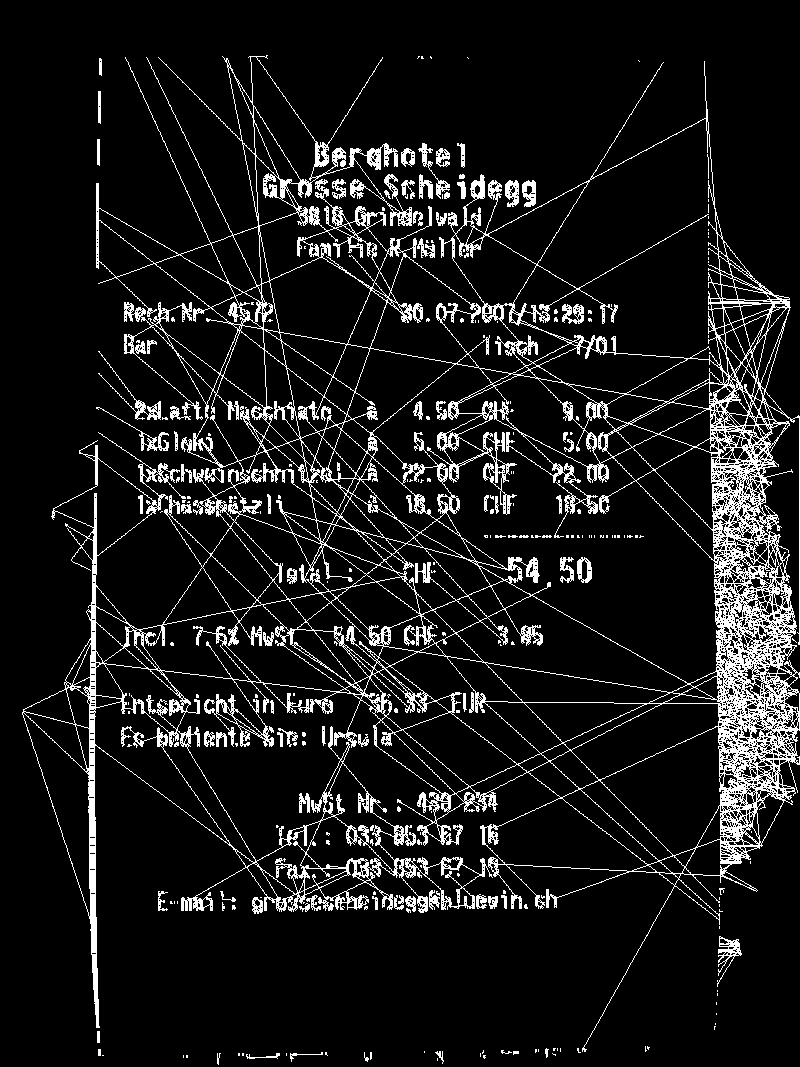
\includegraphics[width=3cm]{res/swt.png}
    \caption{Unfinished SWT}
  \end{subfigure}
  \hspace{5mm}%
  \begin{subfigure}[t]{4cm}
    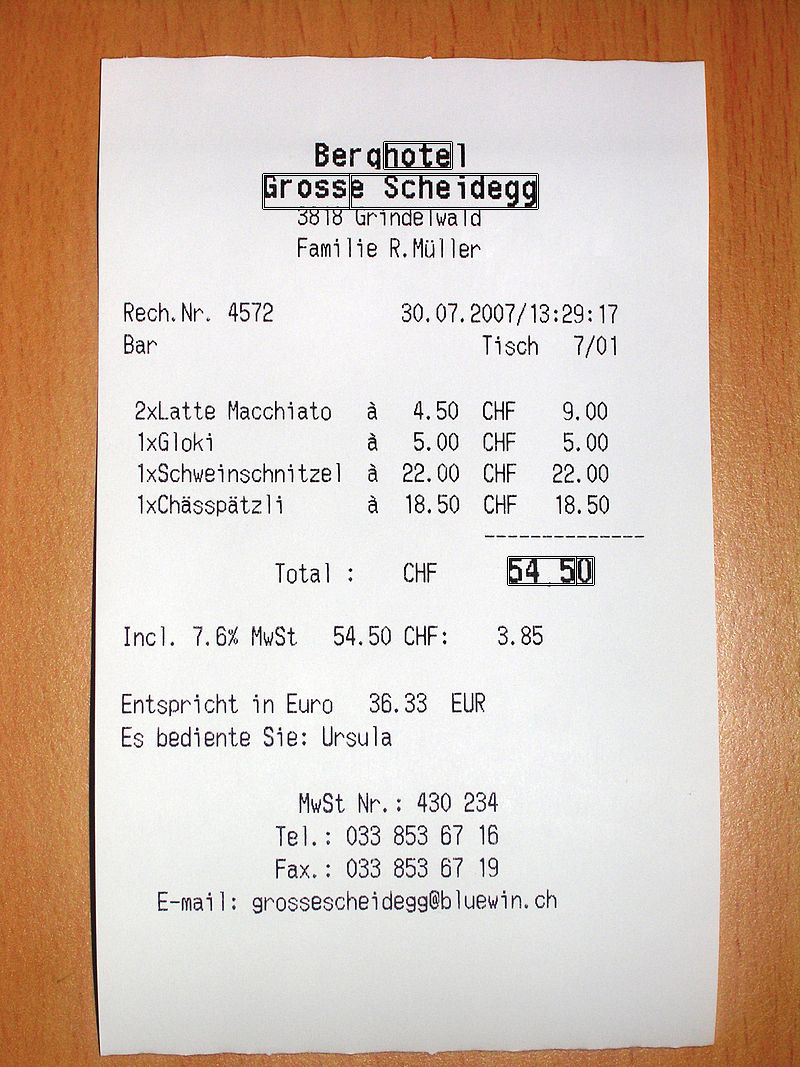
\includegraphics[width=3cm]{res/OpenCV_Std.png}
    \caption{OpenCv Scene text detection}
  \end{subfigure}
  \hspace{5mm}%
  \caption{Result of Discarded Segment Text Method}
  \label{fig:Text_detection_result}
\end{figure}

\section{Preprocessing}
We tried different approaches only on find rotation and character segmentation. Line segmentation and dataset matching we didnt try other methods on.
\subsection{Find rotation}
\label{Discard:rotation}
The original thought was to use the Hough Transform to find the lines in a text, and then from that, find the rotation. However because of bad results, we moved to cv.minAreaRect. This too had some limitations on what it could rotate, see Section~\ref{subsec:Find rotation}. These limitation we tried to solve useing a CNN solution, presented below.

\begin{flushleft}
  \textbf{Discarded Method 1: Hough Transform} \\
  \href{https://en.wikipedia.org/wiki/Hough_transform}{Hough transform} is a well known algorithm to find lines, its approach is to see if it can aligne some threshold of pixels on one straight line. To help with this process we will do a simple edge detection algorithm on the image before running it through the Hough Transform. \par Bellow, the steps needed to perform this approach are mentioned.

  \begin{enumerate}
    \item \textbf{Edge detection}
    Too make the Hough transform perform better we want to remove unnecessary noise. Canny edge detection algorithm is a robust and fast solution for this.
    \item \textbf{Line detection}
    Now perform the actually Hough Transform.
    \item \textbf{Rotate image}
    Lastly we need to rotate the image according to the lines from the Hough Transform.
  \end{enumerate}
\end{flushleft}


\begin{flushleft}
  \textbf{Discarded Method 2: OpenCV minAreaRect() + CNN solution} \\
  This approach builds on the approach presented in Section~\ref{subsec:Find rotation}. As cv.minAreaRect returns text rotated in one of following angles [0\textdegree, 90\textdegree, 180\textdegree, 270\textdegree], see Figure~\ref{fig:4angle_rot} for illustration. We wanted to add a CNN to determine which of the angles is correct and then rotate it accordingly.
  To train the network we needed a dataset with the corresponding angles as labels, as we could not find one, we decided to create it ourselves, see Section~\ref{sec:Datasets} for more on this. \par
  We discarded this approach because it gave only a 65\% accuracy of the right angle, and we are only working on simple text images with little rotation, hence no need for this addition in our software. \par
  The approach is described below:
  \begin{enumerate}
    \item \textbf{OpenCV minAreaRect()}
    The same approach mention in section \ref{Method:Preprocessing} find rotation
    \item \textbf{CNN solution - find correct rotation}
    Now that we have text rotated in one of [0\textdegree, 90\textdegree, 180\textdegree, 270\textdegree], we have several options finding the correct angle of the text segment.
    \begin{enumerate}
      \item{The most straightforward approach would be to find the rotation of first character and rotate the whole segment accordingly (fast and naive)}
      \item{Pick N characters and find their rotation, angle with most matches will be our final angle of rotation. This is somewhat slower (depends on N) but gives us bit more confidence than (a)}
      \item{Finally we can classify the angle of each individual character before we try to determine the correct angle based on the results. This gives us the highest accuracy but on the cost of time/computation power. This is the only approach able to successfully recognize this type of text: (find better example)\LaTeX}
      \end{enumerate}
    \end{enumerate}


    \begin{figure}[H]
      \centering
      
\includegraphics[height=4cm]{res/4angle_rot.png}
      \caption{cv.minAreaRect cannot differentiate between 0\textdegree and 180\textdegree, and 90\textdegree and 270\textdegree}
      \label{fig:4angle_rot}
    \end{figure}

\end{flushleft}


\subsection{Character Segmentation}
\begin{flushleft}
Since we used Projection Histogram to find lines, we can use it to find character segments as well. We started initially to do that, but later switched to the new approach. \par
This approach is similar to Line detection in Section~\ref{subsec:Find_line}. Its weakness is that we may not get the right height of each character, See figure \ref{fig:Project_histogram}, meaning we get more background. This is bad becasue later to match the desired format for classification, the resizing/reshaping makes these empty spaces even larger, and the letters even smaller. Consequently it gets more difficult to classify correctly.
\end{flushleft}

\section{Classification}
\label{sec:Discarded Method:Classification}
\begin{flushleft}
  As mention in Section~\ref{Method:Classification}, we also tried to use MLP to do classification of characters.
  We decided to avoid using MLP in our project as it required lots of training data; is not able to detect spatial or minor rotation changes, e.g. a network trained with MNIST with accuracy over 95\% was doing poorly in recognizing machine-printed characters, even though they were etalon of a perfect input.

  \begin{figure}[H]
    \centering
    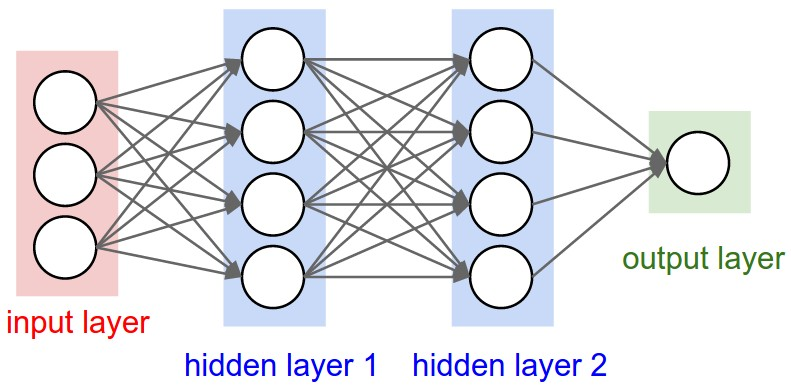
\includegraphics[height=4cm]{res/neural_net2.jpeg}
    \caption{MLP Neural network \href{http://cs231n.github.io/neural-networks-1/}{Source}}
    \label{fig:neural_net2}
  \end{figure}

\end{flushleft}

\section{Datasets}
\label{sec:Datasets}
\subsection{MNIST}
\textit{MNIST} was discarded as we decided to stick with machine printed digits and letters, none of which were included in MNIST. It was a good starting point to test our networks (both MLP and CNN), however to be able to achive a classifier which could classify the english alphabet in addition to numbers ranging from [0-9] we had to go with EMNIST.

\subsection{ROT*}
\textit{ROT*} - dataset containing rotated examples of the same dataset, but with labels corresponding to angle of rotation, e.g. [0, 90, 180, 270]. \par
This dataset was discarded as our network showed very little learning progress as the accuracy of predictions was constantly around 65\%. This is not the datasets fault, most likely it was due to bad network topology or poor choice of hyper parameters but we didn't have enough time to debug this part of the project and decided to stick to OpenCV's minAreaRect() results.


\end{document}
